\documentclass[amssymb,twocolumn,aps]{revtex4}

% allows special characters (including æøå)
\usepackage[utf8]{inputenc}
\usepackage[english]{babel}  %if you write english

\usepackage{physics,amssymb}  % mathematical symbols (physics imports amsmath)
\usepackage{graphicx}         % include graphics such as plots
\usepackage[table]{xcolor}
\usepackage{xcolor}           % set colors
\usepackage{hyperref}         % automagic cross-referencing 
\usepackage{float}			  % force placement of tables and figures

\begin{document}

\title{Report Template \\
    \normalsize FYS-STK3155 - Project X}
\date{\today}
\author{Student}
\affiliation{University of Oslo}

\newpage

\begin{abstract}
    The abstract gives the reader a quick overview of what has been done and the most important results. Try to be to the point and state your main findings. It could be structured as follows:

\end{abstract}

\maketitle

\section{Introduction}
Estimating data has become an invaluable part of both our daily lives and science.
From estimating your heartrate through a smartwatch to predicting the melting of a glacier.
The simplest form of statistical estimation is called \textit{regression}.
Regressin is a method for describing the relationship between one or more independant variables to one dependant variable.
This is done by finding a function or equation that simplifies or estimates the \textit{real} data, thus letting us make estimations about similar data. (source)

While regression analysis is widely used (source), distinguishing different methods could be tricky due to small nuances.
To this end, we will analyze how three regression methods, \textit{Ordinary Least Squares (OLS), Ridge} and \textit{Lasso} estimate Rugne's function, $f(x) = \frac{1}{1 + 25x^2}$.
We will be combining these methods with the \textit{bias-variance tradeoff, cross-validation} and \textit{hyperparameter tuning}, as well as using \textit{bootstrapping} as a resampling method, to find accurate function approximations.

in this article, we will compare the performance of the different methods. We will be using the \textit{Mean Squared Error (MSE)} and \textit{$R^2$-score} to quantify the fit of each method to Rugne's function. 
Firstly, each method, and supporting concepts, will be presented theoretically. Then we will cover the practical implementation of these methods and concepts. Finally, the results are presented and discussed. 



\section{Methods}\label{section:methods}

\subsection{Method 1/X}

\begin{itemize}
    \item Describe the methods and algorithms, including the motivation for using them and their applicability to the problem
    \item Derive central equations when appropriate, the text is the most important part, not the equations.
\end{itemize}

\subsection{Regression}
\subsubsection{OLS}
\subsubsection{Ridge}
\subsubsection{Lasso}
    
\subsection{Gradient decent}
- Standard GD
\subsubsection{Gradient decent with momentum}
\subsubsection{Stochastic gradient decent} 
\subsection{Resampling}
- Hva er resampling
\subsubsection{Bias-variance tradeoff}
\subsubsection{Cross-validation}



\subsection{Implementation}

\begin{itemize}
    \item Explain how you implemented the methods and also say something about the structure of your algorithm and present very central parts of your code, not more than 10 lines
    \item You should plug in some calculations to demonstrate your code, such as selected runs used to validate and verify your results. A reader needs to understand that your code reproduces selected benchmarks and reproduces previous results, either numerical and/or well-known closed form expressions.
\end{itemize}

\subsection{Use of AI tools}

\begin{itemize}
    \item Describe how AI tools like ChatGPT were used in the production of the code and report.
\end{itemize}

\section{Results and Discussion}\label{section:results}

\begin{itemize}
    \item Present your results
    \item Give a critical discussion of your work and place it in the correct context.
    \item Relate your work to other calculations/studies
    \item An eventual reader should be able to reproduce your calculations if she/he wants to do so. All input variables should be properly explained.
    \item Make sure that figures\ref{fig:puppy} and tables contain enough information in their captions, axis labels etc. so that an eventual reader can gain a good impression of your work by studying figures and tables only.
\end{itemize}

\begin{figure}[h]
    \centering
    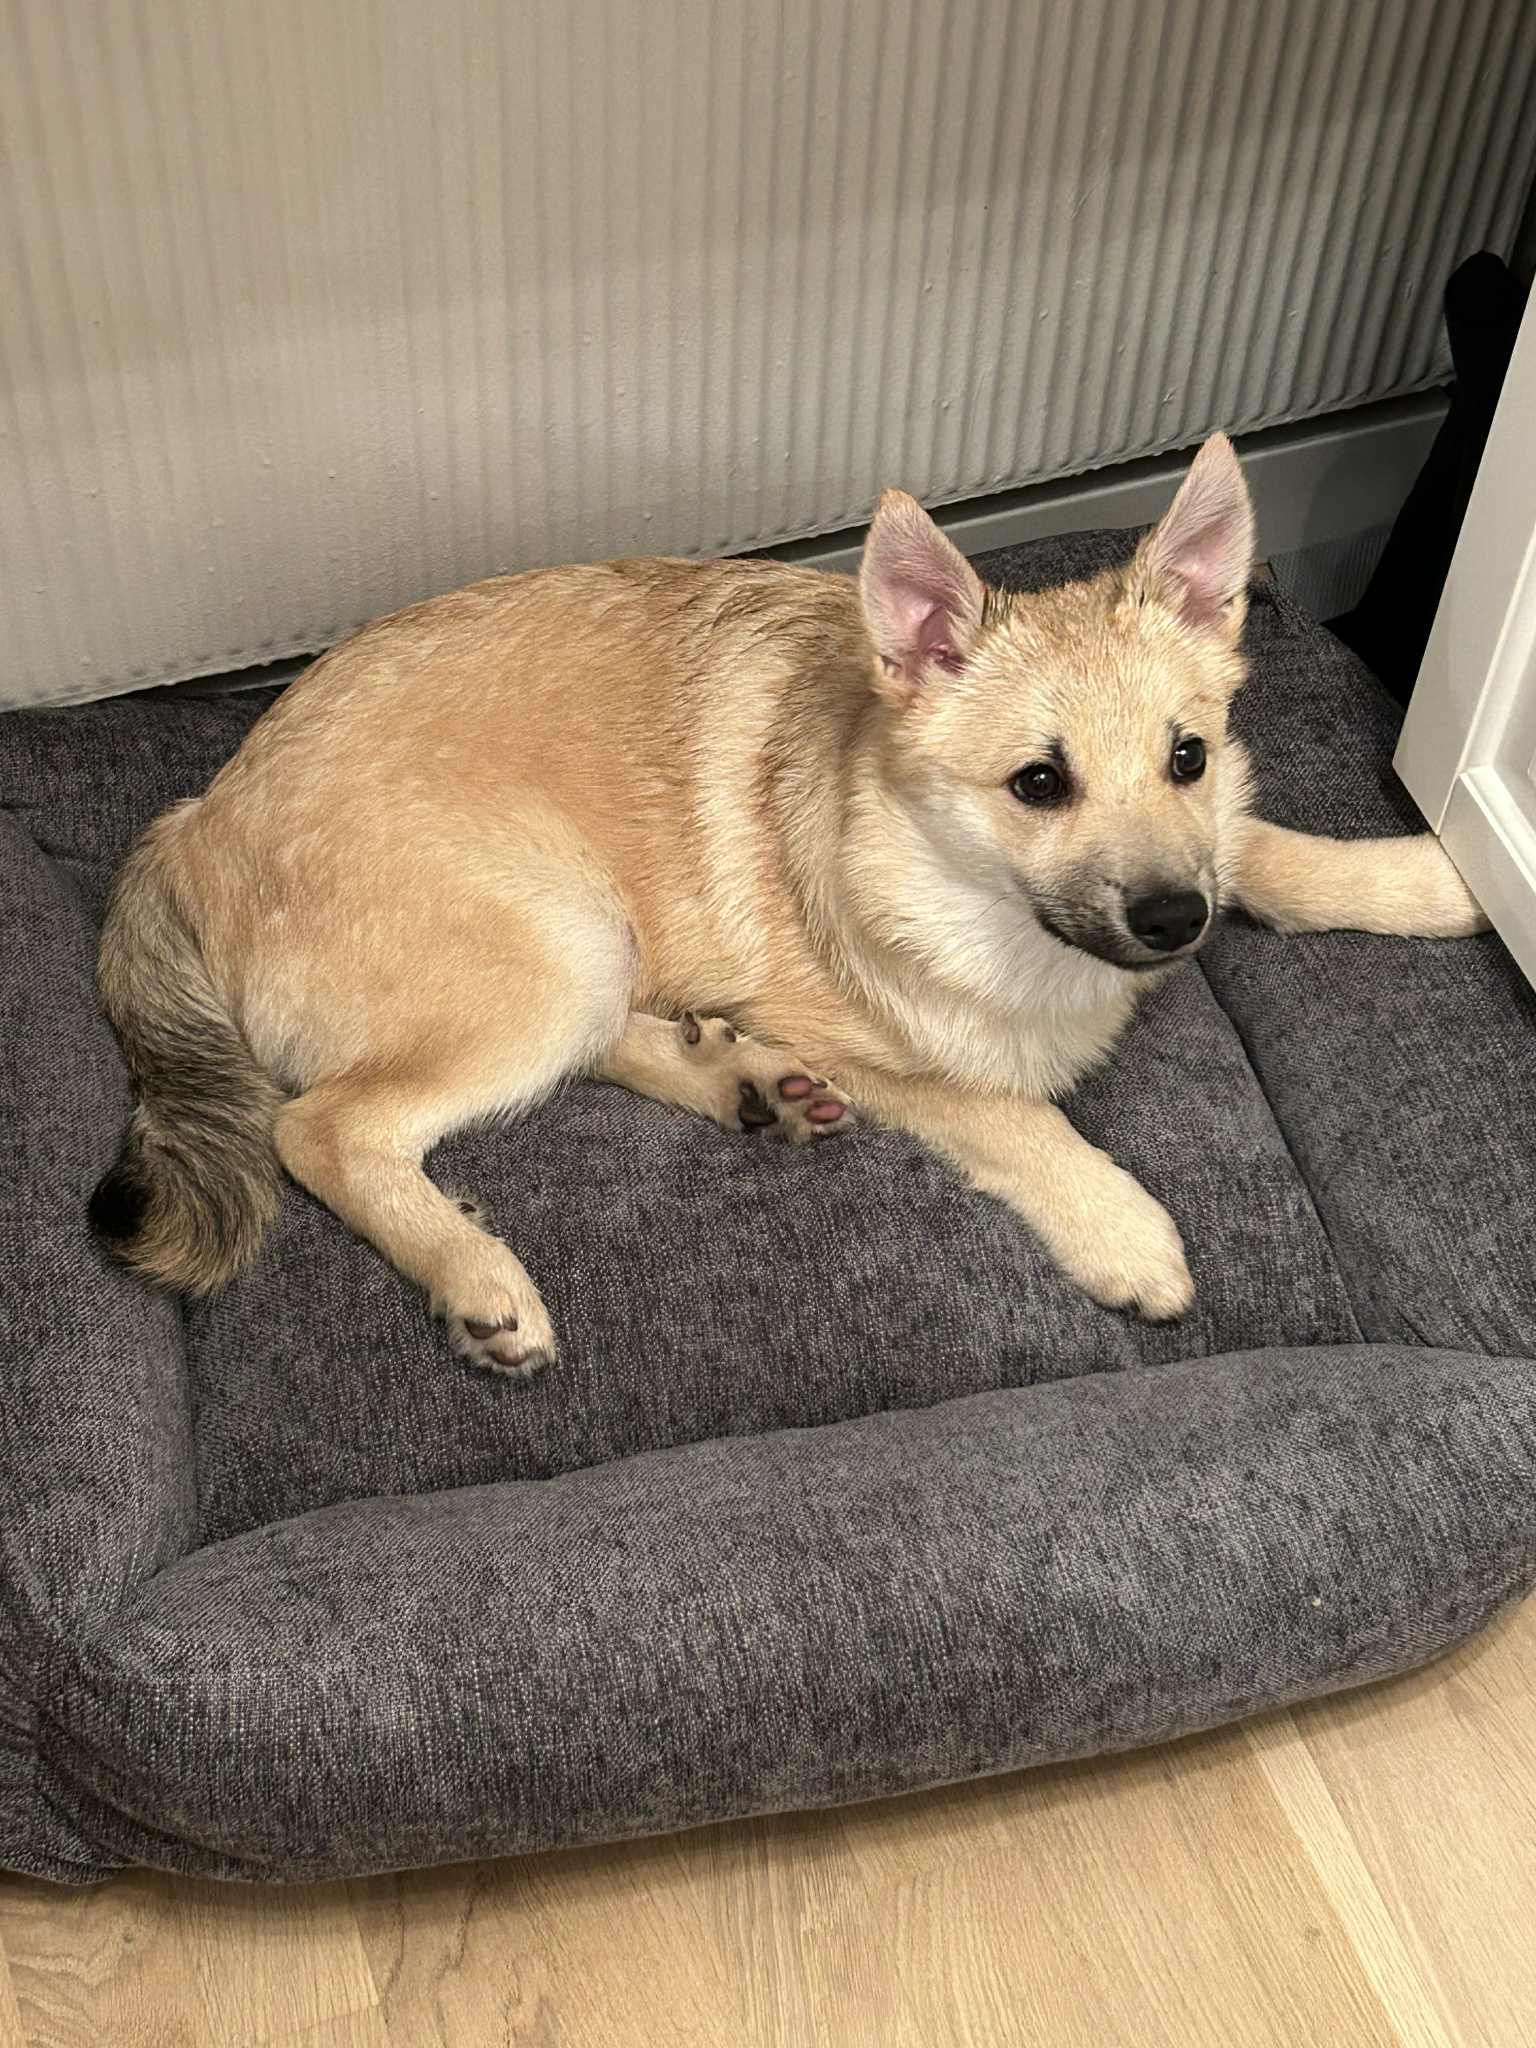
\includegraphics[width=0.5\linewidth]{Figures/puppy.jpg}
    \caption{My dog.}
    \label{fig:puppy}
\end{figure}


\section{Conclusion}\label{section:conclusion}
\begin{itemize}
    \item State your main findings and interpretations
    \item Try to discuss the pros and cons of the methods and possible improvements
    \item State limitations of the study
    \item Try as far as possible to present perspectives for future work
\end{itemize}

\bibliography{biblio}

\end{document}
